\newpage
\section{Exercícios Adicionais}

\paragraph{}
Os exercícios a seguir complementam a lista principal e reforçam a prática dos
métodos de análise vistos em aula, foram retirados de lugares obscuros da
internet (não encontrei de qual livro vieram).

\question{Use nodal analysis to determine the node voltages defined in the
circuit in Fig~\ref{fig:figP3.5}.}
\begin{figure}[H]
  \centering
  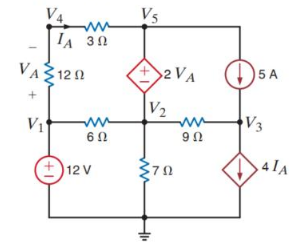
\includegraphics[width=0.4\textwidth]{./fig/figP3.5.png}
  \caption{Exercício Adicional 1}\label{fig:figP3.5}
\end{figure}
\answer{
}

\question{Use nodal analysis to determine the node voltages defined in the
circuit in Fig~\ref{fig:figP3.51}.}
\begin{figure}[H]
  \centering
  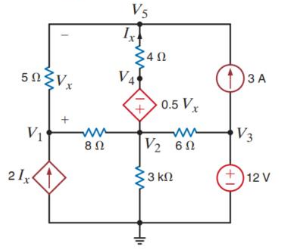
\includegraphics[width=0.4\textwidth]{./fig/figP3.51.png}
  \caption{Exercício Adicional 2}\label{fig:figP3.51}
\end{figure}
\answer{
}

\newpage
\question{Solve for the mesh currents defined in the circuit in
Fig~\ref{fig:figP3.98}.}
\begin{figure}[H]
  \centering
  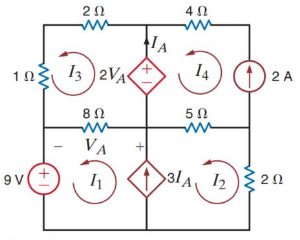
\includegraphics[width=0.4\textwidth]{./fig/figP3.98.png}
  \caption{Exercício Adicional 3}\label{fig:figP3.98}
\end{figure}
\answer{
}
